\chapter{Исследование работы готовых плагинов} \label{ch2}
	
% не рекомендуется использовать отдельную section <<введение>> после лета 2020 года
%\section{Введение} \label{ch2:intro}

Глава посвящена тестированию плагина и поиску ошибок

В параграфе \ref{ch2:title-abbr} приведён процесс и результаты тестирования плагинов в Moodle 3.5. Параграф \ref{ch2:sec-abbr} содержит результат тестирования плагина вопроса в Moodle 3.10. 


\section{Исследование работы плагинов в Moodle 3.5} \label{ch2:title-abbr} %название по-русски

Для наглядного примера работы теста Люшера в системе Moodle была установлена версия 3.5, для которой изначально создавались плагины. 
В ходе первой установки ddlusher\cite{psy-test-ddlusher} система вернула ошибку в инициализации базы данных в файле install.xml: в таблице lusherr содержалось 2 поля с автоматической генерацией значения. После анализа кода стало ясно, что одному из полей не требуется автоматическая генерация при добавлении записи в таблицу, поэтому свойство sequence было снято с поля. Также было исправлено имя таблицы: с mdl\textunderscore lusherr на lusherr, так как при установке плагина система самостоятельно добавляет префикс к названию. После исправлений плагин был успешно установлен.

Плагин lusherr\cite{psy-test-lusherr} установился без ошибок с первого раза. 

Для проверки функционирования был создан курс, тест и вопросы. Тест успешно отработал и вывел результаты: карточки при перемещении на фон исчезали, между вопросами запускался таймер. 


На \firef{fig:res35} приведён скриншот результатов теста.
\FloatBarrier % заставить рисунки и другие подвижные (float) элементы остановиться
	\begin{figure}[ht] 
	\center
	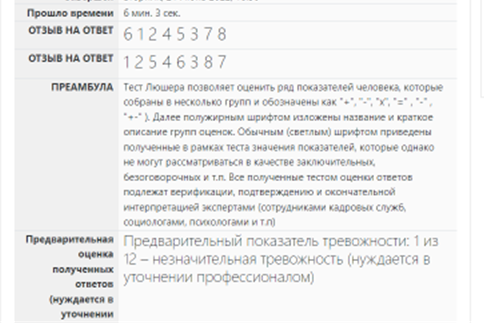
\includegraphics [scale=1.2] {my_folder/images/result35}
	\caption{Результаты теста в версии Moodle 3.5} 
	\label{fig:res35}  
	\end{figure}
\FloatBarrier % заставить рисунки и другие подвижные (float) элементы остановиться
	


	
\section{Тестирование плагинов в Moodle 3.10} \label{ch2:sec-abbr} %название по-русски
Для дальнейшей проверки на компьютере была дополнительно развернута версия 3.10. Установка плагинов прошла без ошибок, однако при попытке создать вопрос в консоли появилась ошибка в файле с Javascript кодом, из-за которой стало невозможно редактировать поля формы. 

На \firef{fig:res310} приведён скриншот результатов теста.
\FloatBarrier % заставить рисунки и другие подвижные (float) элементы остановиться
\begin{figure}[ht] 
	\center
	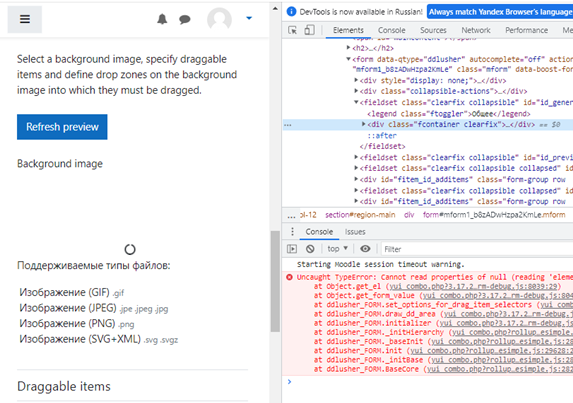
\includegraphics [scale=1] {my_folder/images/result310}
	\caption{Ошибка при попытке создания вопроса в Moodle 3.10} 
	\label{fig:res310}  
\end{figure}
\FloatBarrier % заставить рисунки и другие подвижные (float) элементы остановиться

Плагин поведения протестировать на данном этапе невозможно, так как он зависит от вопроса.
